\begin{quote}
{\em Before EDA, integrated circuits were designed by hand.} -- Daniel Nenni~\cite{wikicite}
\vspace{-2mm}
\end{quote}

\section{Introduction}

Computer networks are growing in scale and complexity, as the world increasingly relies upon them to deliver rich services on demand.  Modern networks are diverse, ranging from data centers that power cloud computing to rural networks.  New applications such as augmented reality and self-driving cars have stringent latency and availability requirements typically associated with large enterprises such as Google with deep pockets and armies of operators. But they also carry over lower tier rural networks (consider a surgeon doing
remote telesurgery in Tamil Nadu) where expertise and money are scarce. And yet our approach to building and maintaining networks has hardly changed in decades.

Networks today are managed using a patchwork of complex, manual, and low-level mechanisms. Network architects produce designs largely by hand, guided by intuition and experience. Network operators reconfigure network devices constantly to match evolving needs, leading to configurations that are inefficient, difficult to understand, and ever more brittle.  Debugging
networked systems and application SLA failures and isolating root causes to  
misconfiguration or component failure is a black art.

As a result, networks today suffer from {\em high cost} (Google~\cite{b4} reports a factor of two underutilization for expensive transoceanic links), {\em high latency} (Amazon~\cite{amazon} asserts that a 100ms increase in latency leads to a 1\% drop in revenue), {\em lack of agility} (a startup~\cite{mahajan} reports that some Fortune 500 companies take over a week to roll out minor configuration changes because they do not fully understand their potential impact), {\em fragility} (surveys~\cite{atpg} have shown that one in three networks have dozens of incidents per month that take over an hour to resolve), and {\em high barriers to entry} (rural networks cannot afford to employ hundreds of highly-trained operators~\cite{barathwisp}). The poor performance and fragility of networks has direct negative impacts on cloud computing. For example, Google aims to limit downtime to ``a few minutes per month''~\cite{rameshgoogle}.

In other fields, increasing scale and requirements led to advances in \emph{design automation}. Hardware designs challenges in the 1970s led to electronic design automation (EDA) as an academic discipline~\cite{alberto} and an industry of EDA tools (e.g., high-level synthesis, functional verification). Similarly, requirements for large-scale software led to high-level languages and companion technologies (compilers, integrated development environments).   McKeown~\cite{mckeown} suggests there is a similar opportunity for network design automation, noting that in both software and chip worlds a \$10B tool industry supports a \$100B software and chip industry, but that networks largely lack such tools. 

Considerable work has been done in design automation for networks in the last five years specifically in {\em network synthesis} and \emph{network verification}.  In 2013, Google~\cite{b4} and Microsoft~\cite{swan} deployed new traffic engineering systems that compute efficient routes through the network automatically and without human intervention. They found that programming the network {\em as a whole} increased utilization and reduced cost by millions of dollars. The community has built tools verification~\cite{veriflow,hsa,lam}, testing~\cite{atpg,nice}, debugging~\cite{xtrace,marple}, topology design~\cite{condor} and designed higher-level languages for expressing network policies~\cite{netkat,propane}.

Compared to EDA, the point solutions listed above are a great start, but there are several gaps: {\em 1. Focus on debugging network configuration not network systems:}  Most work on
network verification~\cite{hsa,veriflow,minesweeper} or synthesis~\cite{netkat,propane} focus
on bugs in router configurations file while other work on debugging \cite{bsd,pathqueries,marple} help identify run-timer performance bugs.  Neither is
connected to the high level systems concerns of operators and developers.  
{\em 2. Focus on data centers:} Most extant work ignores diverse networks such
as rural networks and CDNs. {\em 3. Isolated abstractions:} Existing
abstractions~\cite{netkat,propane,hsa,Ethane,4DControlPlane} are promising but are neither
complete nor interconnected.  {\em 3. Limited outreach:} Existing tools (e.g., Batfish~\cite{batfish}, Propane~\cite{propane} are still not directly
applicable except to expert operators in larger networks.

The goal of this NSF Large is to fill these gaps to move closer to the vision of what we call \emph{Network Design Automation (NDA)}.

\paragraph*{Network Design Automation.}
%
Inspired by the transformative effects of software tools and EDA, we seek to take the next steps towards developing a coherent field of {\em Network Design Automation} (NDA). NDA 
builds on but extends current work in Network Verification and Synthesis based on two
themes that cut across many of the specific research tasks we propose.

{\bf Networked Systems Level Debugging}:  We seek to develop a coherent and interconnected set of tools that map operator and application concerns  to network causes and remedial actions at all time scales from  long term (e.g., detecting failure trends), to compile time (e..g, 
configuration analysis) to run time (e.g., isolating router component failures).  We aim to 
not only extend the state of the art  (e.g., automating operator log insights using NLP instead of
the manual analysis in \cite{rameshgoogle}, finding configuration bugs without a specification
using data mining, tracing application level failures to network problems via machine learning) 
but to \emph{interconnect} these tools and abstractions into a tool for debugging networked
systems.

{\bf Synthesis for a Broader Class of Networks:}: While we will continue to leverage our contacts at Cloud Companies (Google, Microsoft, see letters), to truly democratize the tools we will focus on extending them to other networks (especially rural networks) as part of our goal to allow any network -- big or small - to automate both topology and configuration synthesis.   
We are inspired by Condor~\cite{condor} which used constraint solvers to synthesize an instance of a particular, regular class of topologies (Clos) whose design is independent of traffic matrices.   We will broaden the synthesis problem using constraint solvers to irregular networks where geography, cost, traffic all play a part in the synthesis. While rural networks are our driving example, we will also investigate replica placement in CDNs. Second, while in other
work with David Walker at Princeton~\cite{butane} we are working on top down design of
configurations, we will develop \emph{network scripting} which we feel is a better fit for rural operators and may even generalize to other smaller networks (e.g., home networks, small offices).

{\bf Why Now?} We believe the time is right for NDA, as evidenced by recent progress in academia and industry.  The number of papers on top-down design and verification at SIGCOMM, the flagship networking conference, grew from 1/30 before 2011 to 8/40 in 2016. Veriflow~\cite{veriflow} and Forward Networks~\cite{forward} received millions in venture capital funds in 2015 to verify network properties. In 2015, Cisco founded a design automation unit called Candid under Sundar Iyer~\cite{sundar}, and Amazon hired Byron Cook to create a cloud verification group~\cite{byron}.  While there has been a flurry of recent activity in 
design tools for clouds, initial work has also begun on network design for rural
networks~{barath}.




% \begin{table}
% \begin{small}
% \centerline{
% \begin{tabular}{@{}|@{\,}c@{\,}|@{\,}c@{\,}|@{\,}c@{\,}|@{}}
% \hline
% {\bf Task} & {\bf Abstraction} & {\bf Sample Scientific Question} \\
% \hline High-Speed Packet Forwarding &
% Hardware tile description  &
% Can stochastic search help design hardware? \\
% \hline Flexible Router Compilers & IRs for Packet Processing & What is ``the LLVM'' for routers?\\
% \hline Topology Design & Topology Description Language & Can SAT Solvers aid topology design? \\
% \hline Network Management & Network Policy Language & How to apply stepwise refinement to networks? \\
% \hline Network Monitoring & Performance Query Language & How to map performance assertions to routers? \\
% \hline Failure Analysis & Cause-effect Graphs & Can NLP find causal relations from text? \\
% \hline
% \end{tabular}
% }
% \end{small}
% \caption{Sample tasks, abstractions, and scientific questions for our proposed research on NDA.}
% \label{scientificquestions}
% \end{table}

\begin{figure}[t]
\centerline{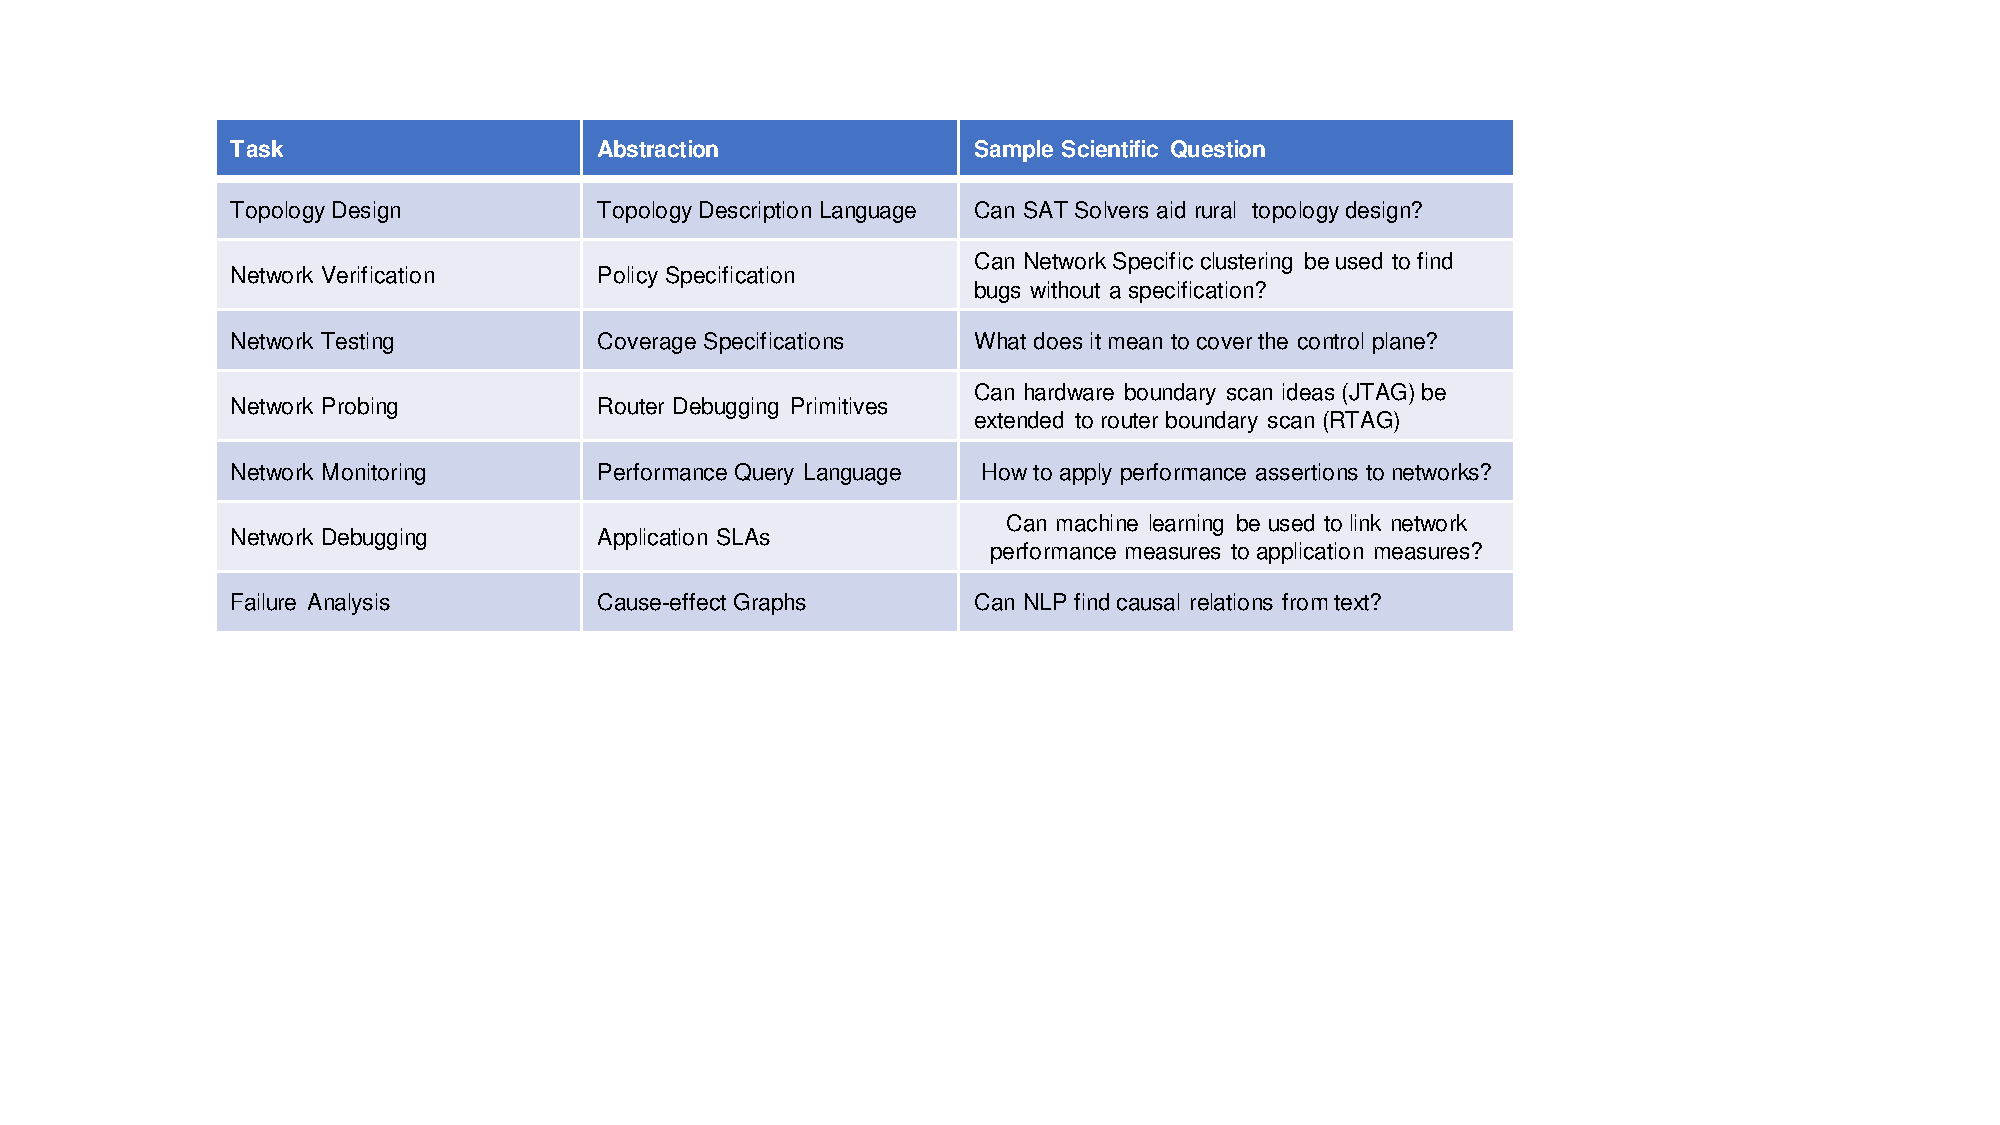
\epsfig{file=questions_table.pdf, height=5in}}
\caption{Sample tasks, abstractions, and scientific questions for our
  proposed research on NDA.}
\vspace{2mm}
\label{scientificquestions}
\end{figure}


\paragraph*{1. Intellectual Merit: NDA Science.} {\em We will develop a science of network design automation that harnesses interdisciplinary approaches but rethinks them to leverage the structure of networks.} One can view a network as either a ``program'' or a hardware circuit that transforms incoming packets at the incoming edge of to output packets.  These lenses suggest adapting tools
for software and hardware synthesis and debugging.  At the same time, recent progress in fields such as supervised machine learning, data mining and natural language processing seem natural techniques to detect failure patterns in networking.  Our experience in network verification, however, has taught us
that effective solutions for network system debugging and synthesis must exploit the stucture of the network domain.  For example, we show in Section~\ref{sec:verification} that attempts to cluster routers into roles using off  the
shelf k-means clustering works badly but more network specific clustering
works well. Table~\ref{scientificquestions} summarizes some of the language design and scientifc questions we will address.

\paragraph*{2. Broader Impact: Network Design Tools.}{\em We will build a suite of tools for networks to begin to catalyze an industry for Network Design Automation akin to the EDA industry.}   
%
 Our vision is that architects at Fortune 500 companies and rural ISPs  can use NDA tools to develop designs in hours or days, lowering cost and increasing robustness. We also envisage network operators to be able to debug complex application problems much faster using our tools.  While we do not propose to deliver industrial-strength tools, we plan to collaborate with established companies (VMWare, Cisco, Google, and Microsoft) and startups (Veriflow and Forward Networks) via internships and joint projects (see letters  attached to this proposal). 

\paragraph*{3. Broader Impact: NDA Education.} {\em We will take first steps toward lowering the educational barriers for people around the world to operate networks.}
%
As with the EDA and software revolutions, achieving wide impact will require educational materials to train the next generation to use NDA methodologies and technologies. To enfranchise operators, we will focus on producing open-source course material based on what we call {\em network scripting} that will teach how to manage the vast majority of simple networks found around the world, together with open-source simulators for easy network testing. We seek to complement existing efforts such as Cisco Academy~\cite{ciscoacademy} that have already had major impact in disadvantaged societies. 

{\bf Why an NSF Large?}  While individual researchers and companies can build impressive point solutions, it takes the efforts of several researchers working in concert to map out the landscape of NDA and define its interconnections (see Figure~\ref{fig:abstractions}) in our two thrusts of rural network synthesis and
debugging networked systems.  Our team brings together networking experts (Varghese, Govindan, both ACM Fellows for networking), with PL expert Millstein (who helped found the nascent field of network verification) and domain experts in ICTD (Raghavan), debugging (Netravali), and computer architecture (Tamir) to facilitate interdisciplinary exploration at a much larger scale than is possible in a smaller NSF grant while being co-located in Los Angeles. 

All six researchers, however, are in Los Angeles at UCLA and USC. Further, many of them have worked together successfully in research teams (e.g., Govindan-Varghese, Govindan-Millstein, Millstein-Tamir-Varghese) over many years and many projects. We believe co-location in Los Angeles facilitates genuine collaboration and frequent in-person meetings with students and PIs, in contrast to the more sprawling and comparitively isolated efforts of other multi-institution proposals.

{\bf Why not Industry?} Companies, which generally operate on short-term schedules dictated by the lifecycles of their products, are not incentived to organize a large-scale effort such as NDA, let alone tackle difficult scientific questions. We are inspired by Berkeley's early development of open-source products (e.g., the VLSI Tarball~\cite{wikicite}) and leadership (e.g., by Sangiovanni-Vincentelli and Newton) for EDA.  Three of us (Govindan, Millstein, Varghese) have been working to help pioneer this area for the last five years; we feel it is time to take the next step to consolidate this field further with the help of two energetic young faculty members (Raghavan, Netravali) and an expert in compute architecture (Tamir).

\paragraph*{Related Efforts and Scope.}
%
First, software-defined networking (SDN) provides a set of basic mechanisms that allow network routers to be centrally programmed.  We contend that NDA is necessary to fulfill the promise of SDN, just as higher-level languages and tools were necessary to fulfill the promise of VLSI. Further, NDA does not depend on SDN. Our focus is on building tools for existing networks in the next 5 years while laying a foundation for the future. Second, while NDA encompasses aspects of security that are directly impacted by network design and operations, such as ensuring isolation and detecting attacks, other aspects of security, such as encryption and authentication, are out of scope for this project.  

Third, we will focus in this grant on verification and automation of 
existing networks as opposed to more clean slate
approaches being pursued by our colleagues at Cornell (Foster) and Princeton (Rexford, Walker).  We fully intend to work with them wherever feasible to look for middle ground. For instance, Millstein and Varghese have an NSF Medium working with Walker at Princeton on making the Propane language more deployable. Fourth, we are all aware of the need for tools such as router compilers for reconfingurable router languages such as  P4~\cite{P4}. However, since tools for router design are cleanly separable from tools for network design, we will focus in this grant on
network tools {\em except} for router hardware debugging primitives to
assist our deep vertical thrust into network system debugging.

All of these extensions (tools for SDN integration, enhancing security, network 
programming language semantics, router compilers) are needed for a complete suite of NDA tools but we do not consider them in this grant to focus our efforts.

